\documentclass[journal]{vgtc}                % final (journal style)
%\documentclass[review,journal]{vgtc}         % review (journal style)
%\documentclass[widereview]{vgtc}             % wide-spaced review
%\documentclass[preprint,journal]{vgtc}       % preprint (journal style)
%\documentclass[electronic,journal]{vgtc}     % electronic version, journal

%% Uncomment one of the lines above depending on where your paper is
%% in the conference process. ``review'' and ``widereview'' are for review
%% submission, ``preprint'' is for pre-publication, and the final version
%% doesn't use a specific qualifier. Further, ``electronic'' includes
%% hyperreferences for more convenient online viewing.

%% Please use one of the ``review'' options in combination with the
%% assigned online id (see below) ONLY if your paper uses a double blind
%% review process. Some conferences, like IEEE Vis and InfoVis, have NOT
%% in the past.

%% Please note that the use of figures other than the optional teaser is not permitted on the first page
%% of the journal version.  Figures should begin on the second page and be
%% in CMYK or Grey scale format, otherwise, colour shifting may occur
%% during the printing process.  Papers submitted with figures other than the optional teaser on the
%% first page will be refused.

%% These three lines bring in essential packages: ``mathptmx'' for Type 1
%% typefaces, ``graphicx'' for inclusion of EPS figures. and ``times''
%% for proper handling of the times font family.

\usepackage{enumerate}

\usepackage{mathptmx}
\usepackage{graphicx}
\usepackage{times}

\usepackage{booktabs}
\usepackage{subfigure}

\usepackage{listings}

%% We encourage the use of mathptmx for consistent usage of times font
%% throughout the proceedings. However, if you encounter conflicts
%% with other math-related packages, you may want to disable it.

%% This turns references into clickable hyperlinks.
\usepackage[bookmarks,backref=true,linkcolor=black]{hyperref} %,colorlinks
\hypersetup{
  pdfauthor = {},
  pdftitle = {},
  pdfsubject = {},
  pdfkeywords = {},
  colorlinks=true,
  linkcolor= black,
  citecolor= black,
  pageanchor=true,
  urlcolor = black,
  plainpages = false,
  linktocpage
}

%% If you are submitting a paper to a conference for review with a double
%% blind reviewing process, please replace the value ``0'' below with your
%% OnlineID. Otherwise, you may safely leave it at ``0''.
\onlineid{0}

%% declare the category of your paper, only shown in review mode
\vgtccategory{Research}

%% allow for this line if you want the electronic option to work properly
\vgtcinsertpkg

%% In preprint mode you may define your own headline.
%\preprinttext{To appear in an IEEE VGTC sponsored conference.}

%% Paper title.

\title{Tree Colors: color schemes for tree structured data}

%% This is how authors are specified in the journal style

%% indicate IEEE Member or Student Member in form indicated below
\author{Martijn Tennekes and Edwin de Jonge}


\authorfooter{
%% insert punctuation at end of each item
\item
Martijn Tennekes, Statistics Netherlands. E-mail: m.tennekes@cbs.nl.
\item
Edwin de Jonge, Statistics Netherlands. E-mail: e.dejonge@cbs.nl.
}

%other entries to be set up for journal
\shortauthortitle{Biv \MakeLowercase{\textit{et al.}}: Hierarchical color palettes}
%\shortauthortitle{Firstauthor \MakeLowercase{\textit{et al.}}: Paper Title}

%% Abstract section.
\abstract{
Color is an important means to display categorical data in statistical graphics. Categories are often hierarchically structured in a classification tree, but most color palettes do not take this hierarchy into account. We present a method to map tree structures to colors from the Hue-Chroma-Luminance (HCL) color model. The HCL color space is known for its well balanced perceptual properties. Our study suggest that hierarchical qualitative color palettes are very useful: not only for improving standard hierarchical visualizations such as trees and treemaps, but also for showing tree structure in non-hierarchical visualizations.
} % end of abstract

%% Keywords that describe your work. Will show as 'Index Terms' in journal
%% please capitalize first letter and insert punctuation after last keyword
\keywords{Color palettes, statistical graphics, hierarchical data.}

%% ACM Computing Classification System (CCS). 
%% See <http://www.acm.org/class/1998/> for details.
%% The ``\CCScat'' command takes four arguments.

\CCScatlist{ 
 \CCScat{H.5.2}{ Information Interfaces and Presentation}%
{User Interfaces}{User-centered design}
}


%% Uncomment below to include a teaser figure.
  \teaser{
  \centering
 \mbox{\subfigure{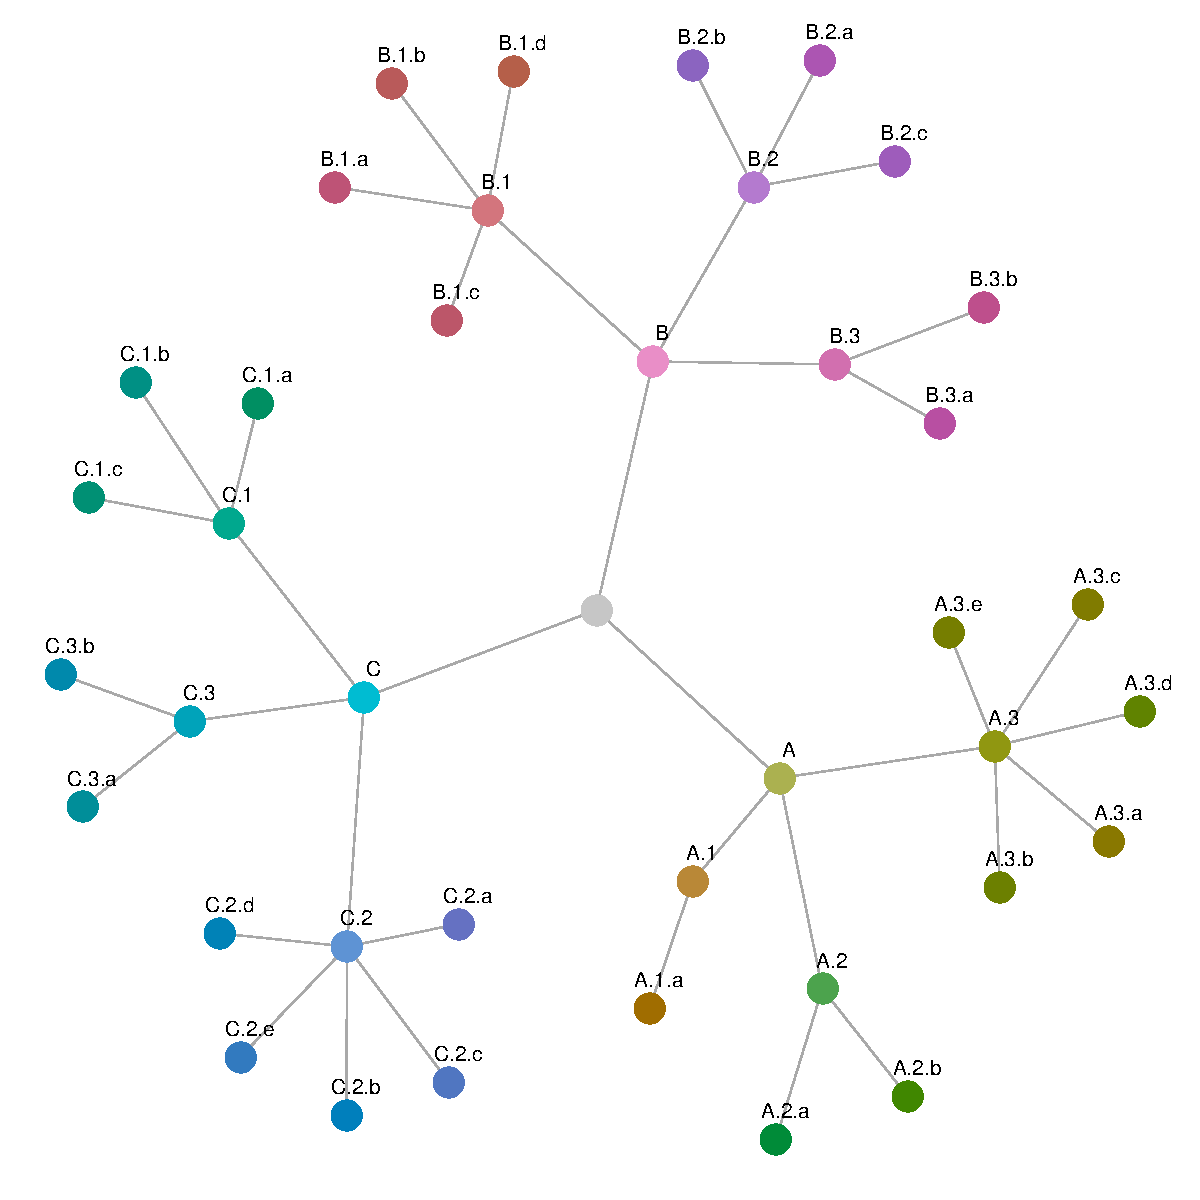
\includegraphics[width=8cm]{Graph_teaser.pdf}}\quad
  \subfigure{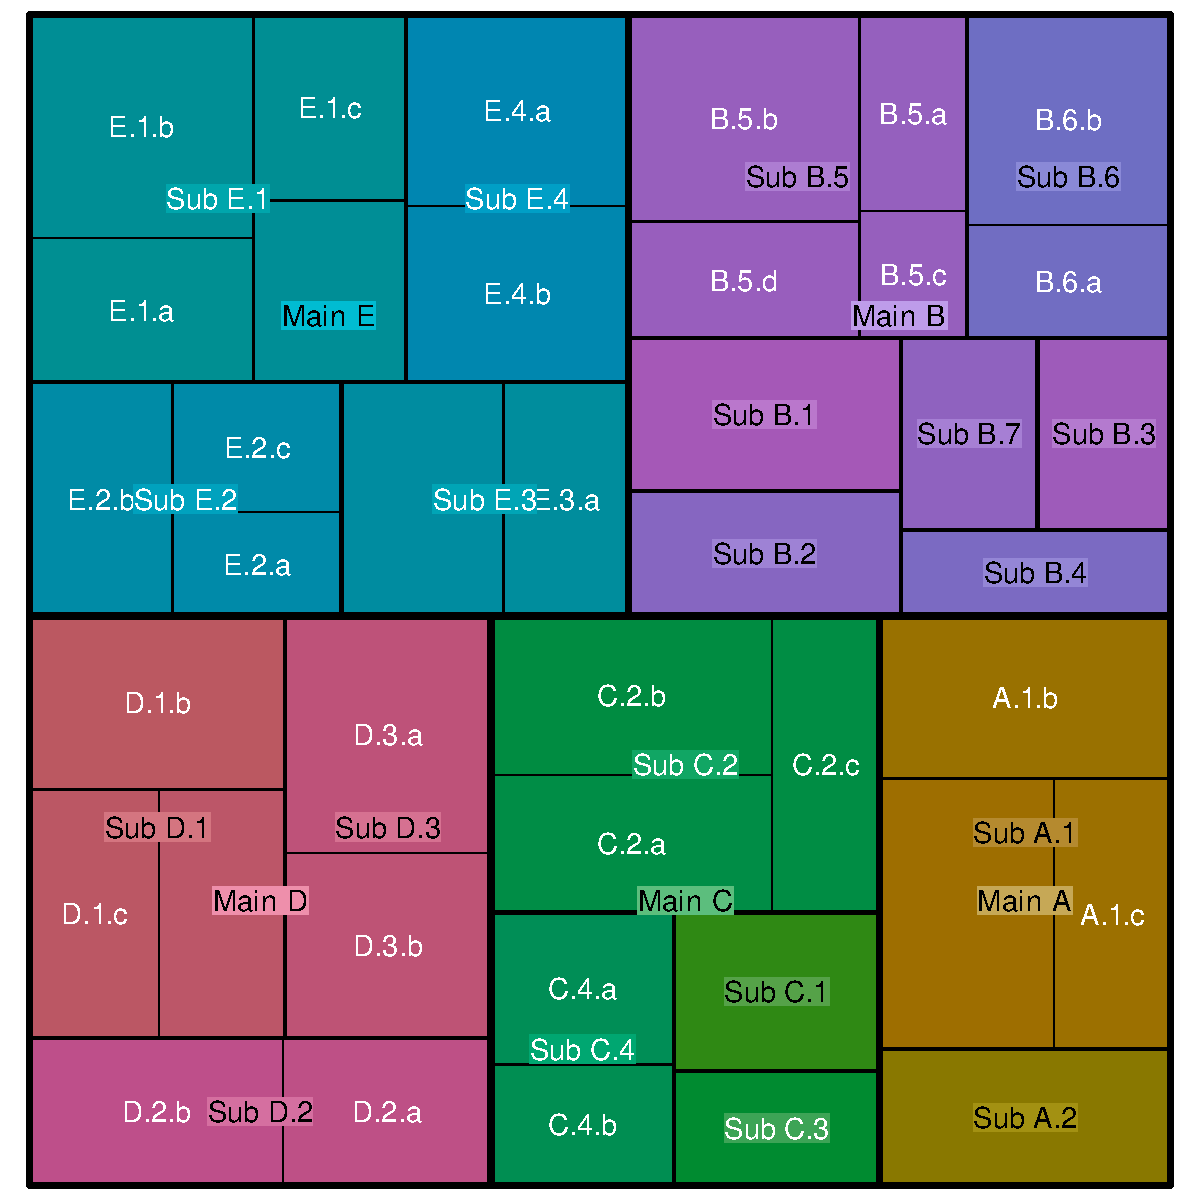
\includegraphics[width=8cm]{Treemap_teaser.pdf}}}
  \caption{Tree Colors applied to a directed graph (left) and a treemap (right).}\label{fig:teaser}
  }

%% Uncomment below to disable the manuscript note
%\renewcommand{\manuscriptnotetxt}{}

%% Copyright space is enabled by default as required by guidelines.
%% It is disabled by the 'review' option or via the following command:
% \nocopyrightspace

%%%%%%%%%%%%%%%%%%%%%%%%%%%%%%%%%%%%%%%%%%%%%%%%%%%%%%%%%%%%%%%%
%%%%%%%%%%%%%%%%%%%%%% START OF THE PAPER %%%%%%%%%%%%%%%%%%%%%%
%%%%%%%%%%%%%%%%%%%%%%%%%%%%%%%%%%%%%%%%%%%%%%%%%%%%%%%%%%%%%%%%%


\graphicspath{{../plots/}}


\begin{document}

\lstset{language=R}
%% The ``\maketitle'' command must be the first command after the
%% ``\begin{document}'' command. It prepares and prints the title block.

%% the only exception to this rule is the \firstsection command
\firstsection{Introduction}

\maketitle

Hierarchical data are of crucial importance in official statistics. Most published data follow a hierarchical classification, for instance broken down by geographic regions or economic activities. To produce statistics it is therefore important to expore and visualize rough input data in a hierarchically structured manner. Several data visualization methods are useful for this task, for instance treemaps
\cite{shneiderman1992,tennekes2011b}. Color palettes reflecting the hierarchical structure would be very useful in supporting visual analysis.

Assigning colors to categories is far from trivial. On the one hand, qualitative colors should be distinct, but on the other hand they should not suggest non-existent order or proximity and introduce perceptual bias. The selection of color palettes for categorical data first depends on the type of data. For nominal data, such as gender or nationality, qualitative color palettes are used, while for ordinal data, such as level of urbanization, sequential or diverging palettes are used \cite{brewer03, zeileis2009}. However, for hierarchical categories there are no specific guidelines for selecting color palettes, to the best of our knowledge.

Although many tree visualizations are proposed in literature \cite{schulz2011}, most of them use color to a small extent. A visualization technique that uses color as a major attribute is the InterRing \cite{yang2002}, a navigation tool with a radial layout. The leaf nodes are assigned to a different hue values. The color of a parent node is derived from averaging the colors of its children, where larger branches have more weight. An implicit effect is that colors of higher hierarchical levels are less saturated, except for one-child-per-parent branches. Hierarchical color schemes are also applied to the Hyperbolic Wheel \cite{lam2012}, an exploration tool for hierchical data.  These color schemes are abstracted from the Hue-Saturation-Lightness (HSL) space, where brightness decreases proportional from root to leaf nodes, and where child nodes inherit the hue values from their parent nodes and add small hue values to distinct them from their siblings. However, hue values of nodes in the same hierarchical layer may be overlapping.

Our purpose is to map tree structures to color palettes with the following three properties. First, the hierarchical depth of a node should be perceived with color. The second property is that branches should be clearly distinguishable in all parts of the tree, or at least the main branches in large trees. Third and last, each node should have a unique color that is also perceived as unique as much as possible.

The color palettes that are obtained by our proposed method are called Tree Colors. As a starting point, we use the Hue-Chroma-Luminance (HCL) space, a transformation of the CIELUV color space, that is designed with the aim to control human color perception~\cite{ihaka2003}. Colors with different hue values are perceptually uniform in colorfulness and brightness, which does not hold for the popular Hue-Saturation-Value (HSV) and HSL color spaces~\cite{zeileis2009}.

This paper is outlined as follows. In Section~\ref{secmethod} we describe the proposed method. We provide several applications of statistical graphics that use Tree Colors in Section~\ref{secapplication}. The conducted user survey to evaluate the method is described in Section~\ref{secuser}. We conclude with a discusssion in Section~\ref{secdisc}.

\section{Method}\label{secmethod}
Our method maps a tree structure on colors in HCL space, such that it reflects the hierarchical properties of the tree. We use the hue parameter $H$, with range [0, 360], for the tree structure, where the hue of each child node resembles the hue of its parent. The chroma and lumnience parameters $C$ and $L$, both with range [0, 100], are used to discriminate the different hierarchical levels.

We illustrate Tree Colors with a radial tree graph that is depicted in Figure~\ref{fig:graph}. Although other graph layouts may be more suitable to highlight the tree structure, for instance the Fruchterman-Reingold algorithm~\cite{Fruchterman91} applied in the graph in Figure~\ref{fig:teaser}, the applied radial Reingold-Tilford layout~\cite{reingold81} preserves the original order of nodes in each hierarchical layer, which is in many cases, and also in this case, purely alphabetical. The Tree Colors in this graph can therefore be applied in the same order in any other visualization method with a radial layout, or a  layer-wise linear layout. %Radial layouts have proven to be very useful in many tree visualizations methods and navigation tools \cite{schulz2011}.

\begin{figure}[htb]

  \centering
  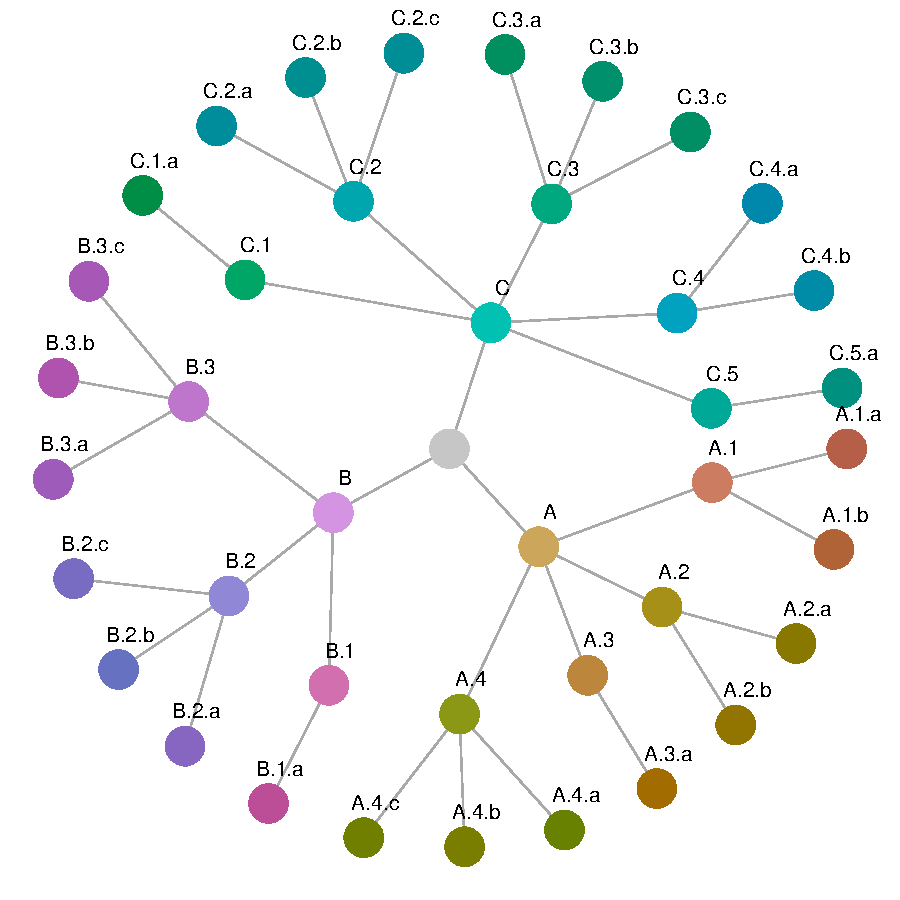
\includegraphics[width=3.2in]{HCPgraph.pdf}
  \caption{Radial graph with Tree Colors.}\label{fig:graph}

\end{figure}

\subsection{Hue values}

For selecting hue values we use the following recursive algorithm. It will assign to each node $v$ of a tree structure a hue value $H$ and a hue value range $r$.
We start with the root node, which has by default hue range $[0, 360]$:

\smallskip{\bf AssignHue($v$, $r$)}
\begin{enumerate} \itemsep1pt \parskip0pt 
\parsep0pt
\item Assign the middle hue value in $r$ to $H$ \footnote{The root node itself is colored grey, so its hue is irrelevant.}.
\item Let $N$ be the number of child nodes of $v$. If $N>0$ :
\begin{enumerate}[i] \itemsep1pt \parskip0pt 
\parsep0pt
\item divide $r$ in $N$ equal parts $r_i$;
\item permute the $r_i$'s and assign them to the child nodes;
\item reduce each $r_i$ by keeping the middle fraction $f$;
\item for each child node $v_i$ DO AssignHue($v_i$, $r_i$).
\end{enumerate}
\end{enumerate}

\begin{figure}[htb]
  \centering
  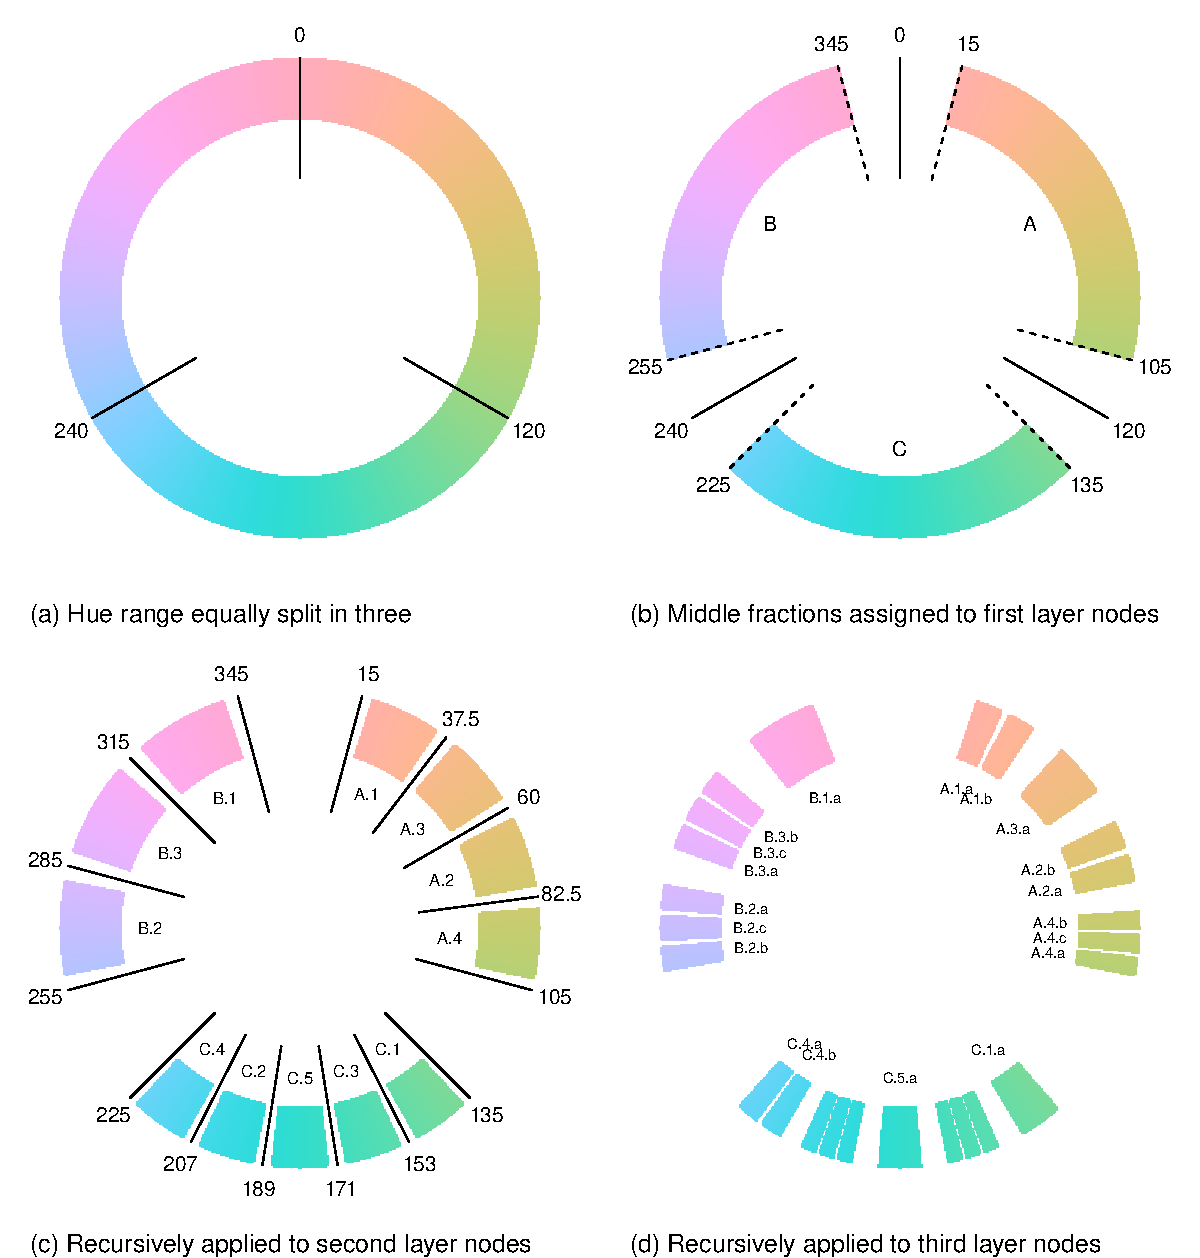
\includegraphics[width=3.5in]{hcl_method2.pdf}
  \caption{Assignment of hue values.}\label{fig:wheel}
\end{figure}

This algorithm is illustrated in Figure~\ref{fig:wheel}. In (a) the full hue range (for a constant $C=60$ and $L=70$)  is divided and permuted among the three children of the root, A, B and C. For these three ranges, the middle fractions (with $f=0.75$) are kept in (b).
In (c) and (d) these steps are recursively taken for the deepest two hierarchical layers.

In many hierarchical structures, there is no order between siblings. When the nodes in such structure are plotted in a linear or radial layout, the colors of the siblings should not introduce a perceptual order. Therefore, the assigned hue ranges are permuted among the siblings. The used permutation order is based on the five-elements-permutation $[1, 3, 5, 2, 4]$. The way to determine the permuted order is to equally spread the siblings on a circle in the original order, and to pick the siblings at angles of 0 modulo 144 degrees. Notice that the difference of any two adjacent siblings in $[1, 3, 5, 2, 4]$ is exactly $2/5 * 360=144$ degrees, also between the last and the first sibling. For the cases with more than five siblings this picking angle is rounded down if needed. It may occur that a sibling is picked twice while othershave not yet been picked, for instance when 360 is a multiple of the rounded picking angle. In these cases, the next sibling is picked and the process continues with the same picking angle. For the three and four siblings case we use the permutations $[1, 3, 2]$ and $[1, 3, 2, 4]$ respectively. 

The permutations for three to twelve siblings for a hue range between 120 (green) and 240 (blue) are depicted in Figure~\ref{fig:perm}. Note that the order of the five-siblings case, which is [1, 3, 5, 2, 4], is the position of the siblings A, B, C, D, and E respectively. Therefore, the permutation of them is A, D, B, E, and C. 

\begin{figure}[htb]
  \centering
  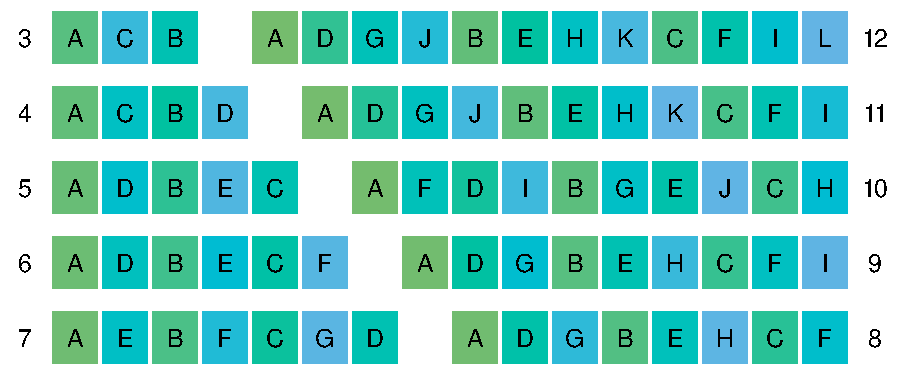
\includegraphics[width=3.5in]{Permutations.pdf}
  \caption{Purmutations of siblings.}\label{fig:perm}
\end{figure}

Furthermore, the permutation within even numbered branches is reversed to differentiate between branches. Note the labeling in Figure~\ref{fig:wheel} shows that the assignment of colors is permuted. The result of the permutation is that siblings are discriminated in each hierarchical layer, which is illustrated in Figure~\ref{fig:graph}.


\subsection{Chroma and luminance values}

In order to show depth in the tree, we use bright colors for nodes high in the tree and dark colors for nodes lower in the tree. The intuition behind this approach is that dark colors are often assiciated by humans with high particle densities. In most tree representations, the density of nodes will increase with the depth of the tree. Therefore, we let luminance decrease linearly with depth.  We set the default luminance value for the first (highest) layer below the root as $L_1=70$. For the other layers $i=2,\ldots, k$, the luminance value is defined as
\begin{equation}
L_i=(i-1)\beta^L + L_1,
\end{equation}
where the default value for the slope parameter $\beta^L$ is set to $-10$. In case the root node is visualized, it is colored grey. Its luminance value of the root node is specified by $L_0=L_1-\beta^L$.

\begin{figure}[htb]
  \centering
  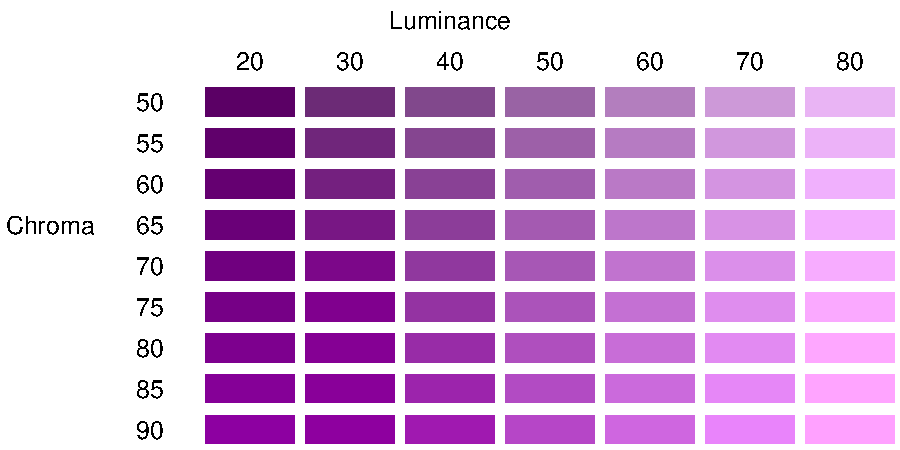
\includegraphics[width=3.5in]{LC.pdf}
  \caption{Colors for different $L$ and $C$ values with a constant $H=300$.}\label{fig:lc}
\end{figure}

In Figure~\ref{fig:lc} a table of colors are depicted for various chroma and luminance values and a constant hue of $H=300$. Brighter colors (with higher values of $L$) have the tendency to become too saturated in our opinion, for instance, the colors with $L=70$ and $C\geq70$. However, for dark colors, high values of $C$ may help to discriminate them distinguigh them from other dark colors with different hue values. The question therefore is, what values of $C$ are needed for what values of $L$ in order to distinguish the colors easily without using too much saturation.


\begin{figure}[htb]
  \centering
  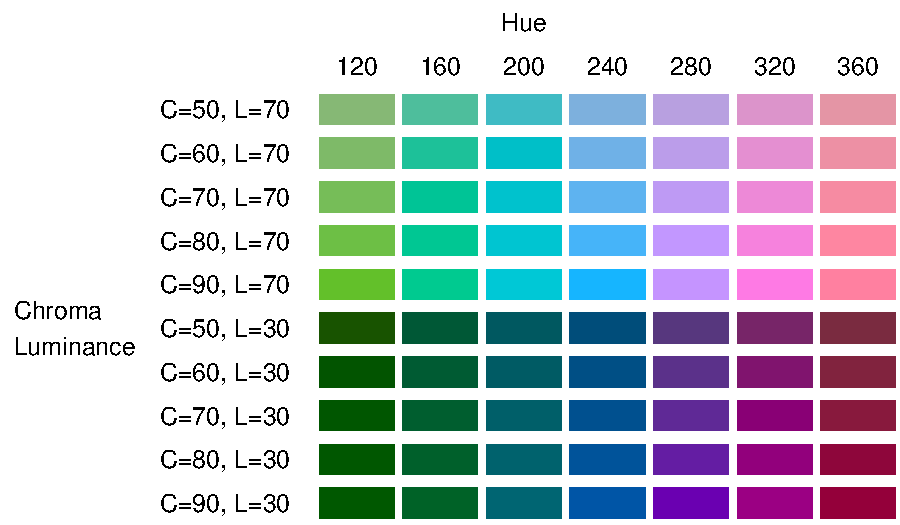
\includegraphics[width=3.5in]{LC2.pdf}
  \caption{Colors palettes for different pairs of $L$ and $C$.}\label{fig:lc2}
\end{figure}

For different pairs of $C$ and $L$, color palettes with a fixed hue range from 120 and 360 are depicted in Figure~\ref{fig:lc2}. Among the bright color palettes (with $L=70$) the saturation level of $C=60$ is sufficient to distriminate the colors easily. For the dark color paletetes (with $L=30$), saturation values of $C=80$ or higher are not superfluous, especially because the assigned hue range is often very narrow for nodes low in the tree.

Therefore, we propose to increase $C$ with depth. Let $C_1=60$ be the chroma value for the first layer. For layer $i=2,\ldots, k$, the chroma value is defined as
\begin{equation}
C_i=(i-1)\beta^C + C_1,
\end{equation}
where the slope parameter is set to $\beta^C=5$ by default. The chroma value for the root node is irrelevant, since it is colored grey.

So per hierarchical layer $i$, we have specified a fixed pair of $L_i$ and $C_i$. For these pairs, we depicted color palettes with a fixed hue range between 120 and 360 in Figure~\ref{fig:lc3}.

\begin{figure}[htb]
  \centering
  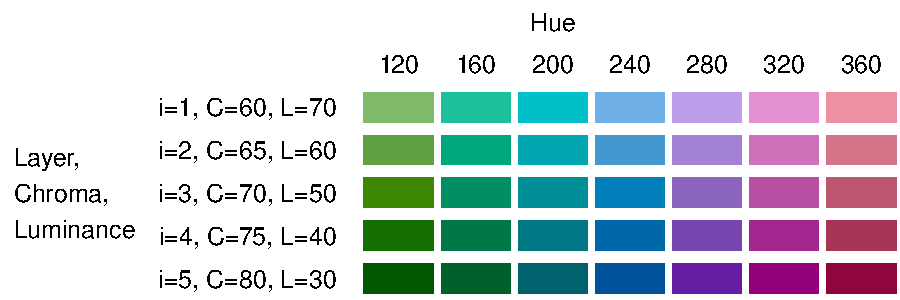
\includegraphics[width=3.5in]{LC3.pdf}
  \caption{Colors palettes for matched pairs of default $L$ and $C$ values for the top five hierarchical layers.}\label{fig:lc3}
\end{figure}

\subsection{Hue fraction}\label{secf}

The fraction $f$ is needed to introduce a `hue gap' between nodes with a different parent. This choice is a trade-off between discriminating different main branches and discriminating different leaf nodes. If $f=0$, the hue ranges are diminished to single hue points, which implies that each main branch is assinged a constant hue. On the other end of the extreme, if $f=1$, the full hue range is available at each hierarchical layer, which makes leaf nodes easier to distinguish, but harder to take apart from leaf nodes of other branches.

\begin{figure}[htb]
  \centering
  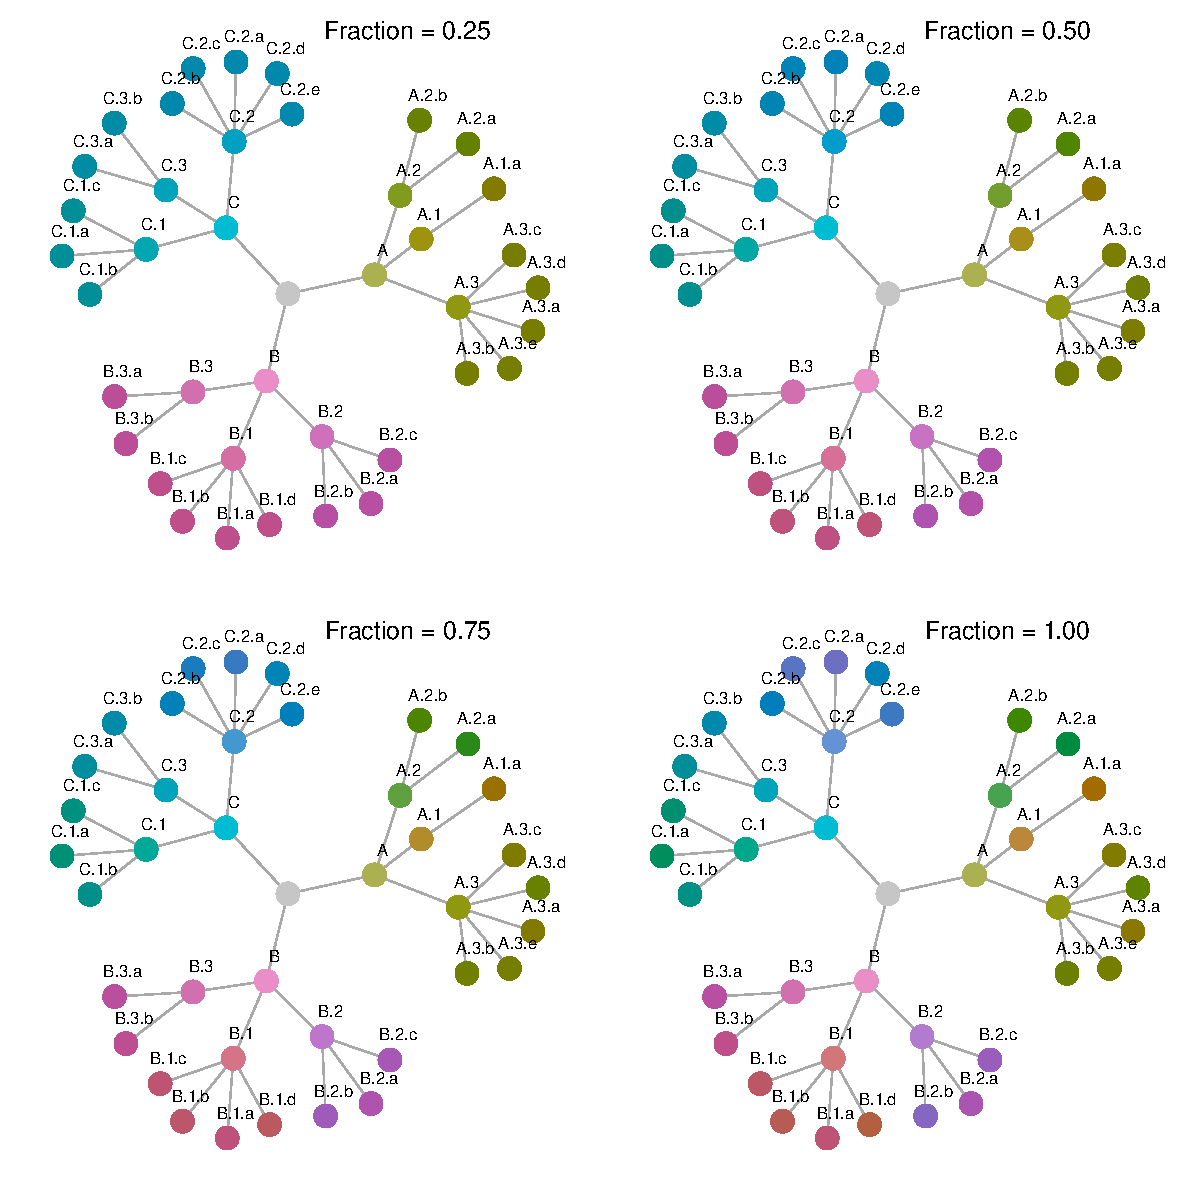
\includegraphics[width=3.5in]{Graph_hue.pdf}
  \caption{Graphs with different fraction values.}\label{fig:graphf}
\end{figure}

The choice of $f$ depends on several aspects, such as the application, the size and dimensions of the hierarchical data, and on the used visualization method. In Figures~\ref{fig:graphf} a graph with a Fruchterman-Reingold layout~\cite{Fruchterman91} is shown with different values of $f$. For such explicit tree visualizations, high values of $f$ can be chosen to discriminate the leaf nodes without loosing tough of the global tree structure which is clearly visible, also without Tree Colors. Even values of (or close to) $1.00$ are appropriate here. To be on the save side, we suggest $f=0.75$ for explicit tree visualizations as a guideline.

\begin{figure}[htb]
  \centering
  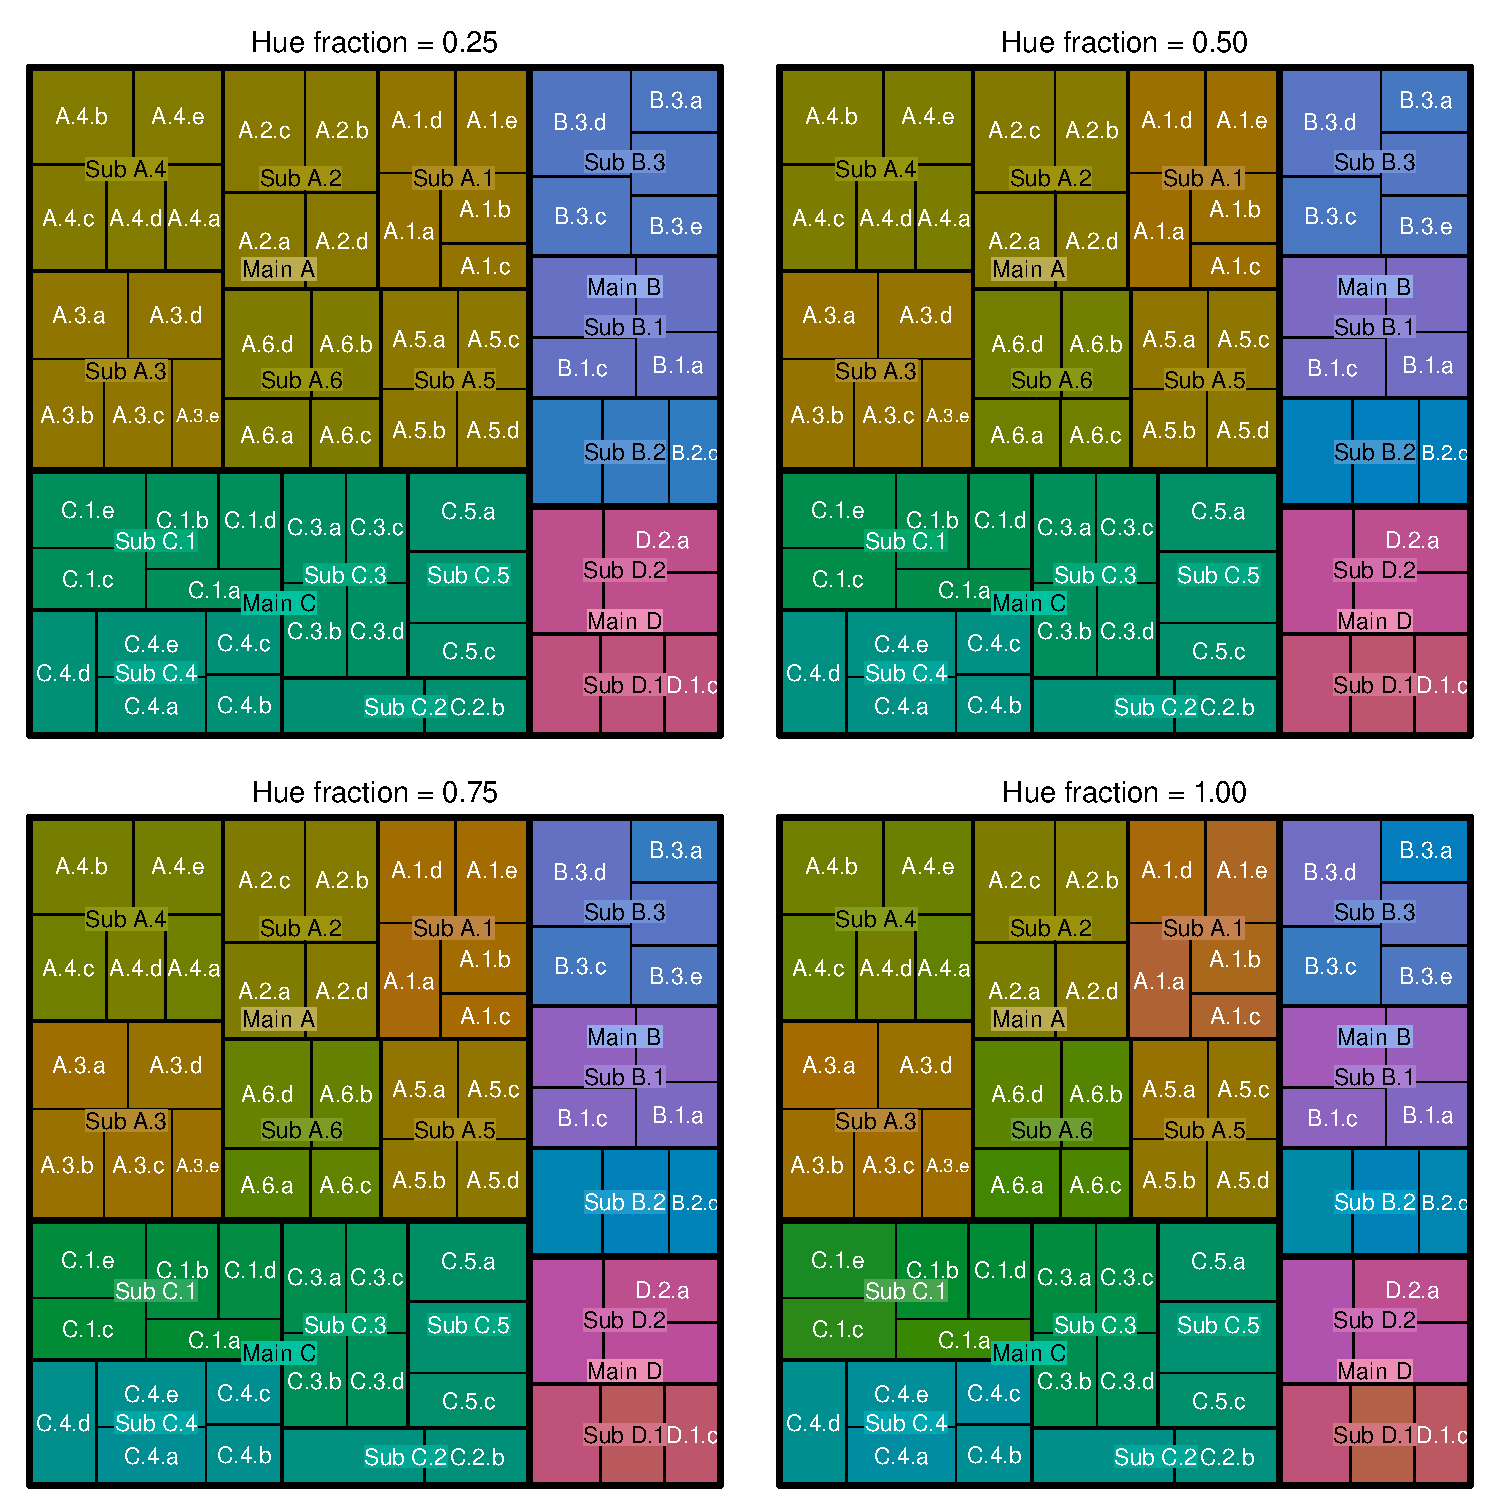
\includegraphics[width=3.5in]{Treemaps_hue.pdf}
  \caption{Treemaps with different fraction values.}\label{fig:treemapf}
\end{figure}


For implicit tree visualizations where the tree structure is not clearly visible without colors, lower values of $f$ are more suitable. To illustrate this, a treemap with different values of $f$ is depicted in Figure~\ref{fig:treemapf}. For $f=0.75$ and especially $f=1.00$, it is difficult to grasp the global tree structure immediately; the main categories A and C are hard to take apart as well as the categories B and D. Therefore we suggest $f=0.50$ as a rule of thumb for implicit tree visualizations.

\section{Software}

A free and open source software tool is available to experiment with the different parameter settings described above. This tool is contained in the software package treemap~\cite{treemap} of the statistical software environment R~\cite{r2013}. After installation R and the package treemap, only two lines of code are required to  start the interactive tool:
\begin{lstlisting}
library(treemap)
treecolors()
\end{lstlisting}

A screenshot is shown in Figure~\ref{fig:screen}.

\begin{figure}[htb]
  \centering
  \fbox{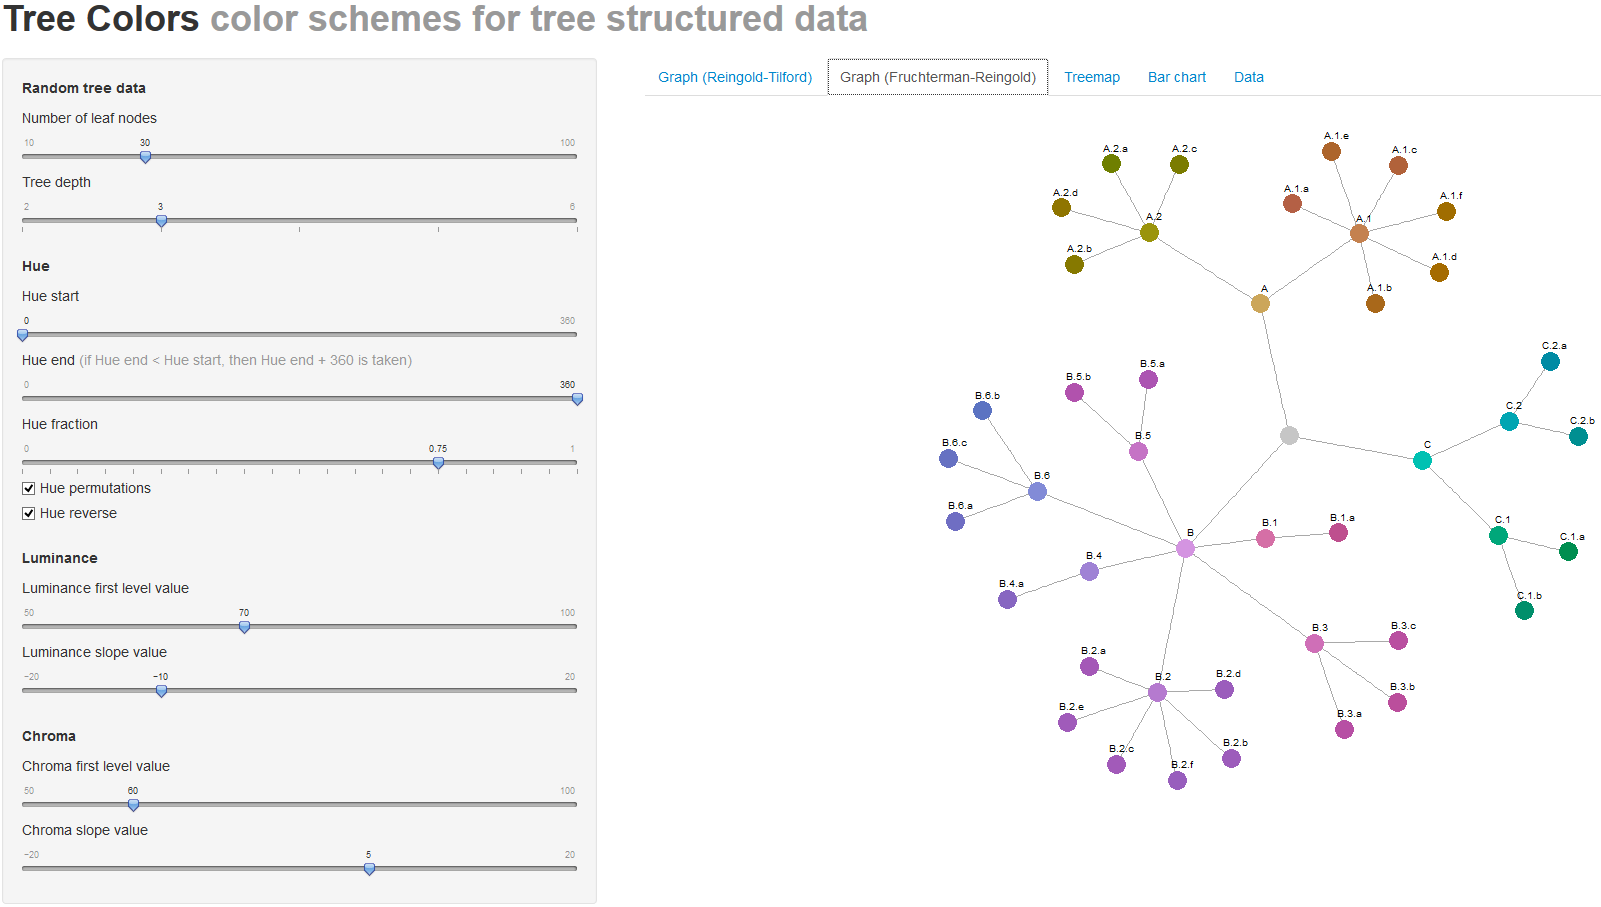
\includegraphics[width=3.5in]{screenshot_treecolors.png}}
  \caption{Screenshot.}\label{fig:screen}
\end{figure}



\section{Application}\label{secapplication}
The hierarchical colors can be applied to enhance standard tree visualizations, as we saw in Figure~\ref{fig:sbiF}. Strictly speaking this is redundant color usage, but in our opinion it can improve many tree visualizations, because branches can be distinguished more easily. 

A second example of improvement is depicted in Figure~\ref{fig:treemapF}. It shows a treemap depicting (fictious) turnover values in Construction (NACE F). In official statistics, turnover is available for each business enterprise in a business register, and aggregated according to the NACE tree. The hierarchical color palette is used to differentiate between different aggregated groups, that makes it possible to compare turnover values at different hierarchical layers. Although the colors of higher NACE layers are only used for the text label backgrounds, they are also resembled by the colors of the lowest NACE layers. This treemap is created with the free and open source R package treemap \cite{treemap}.

Hierarchical colors can also improve visualizations without explicit tree structure. The colors hint at the underlying tree structure.
To illustrate this, a bar chart and a stacked area chart of fictive turnover data are depicted in Figure~\ref{fig:charts}. Such graphics could be useful when the hierarchical structure will not be the main focus in the conducted analyses. The bar chart can be used to compare turnover values of all leaf node sectors in Construction (NACE F), and the stacked area plot to analyse turnover values in time.





\begin{figure}[htb]
  \centering
  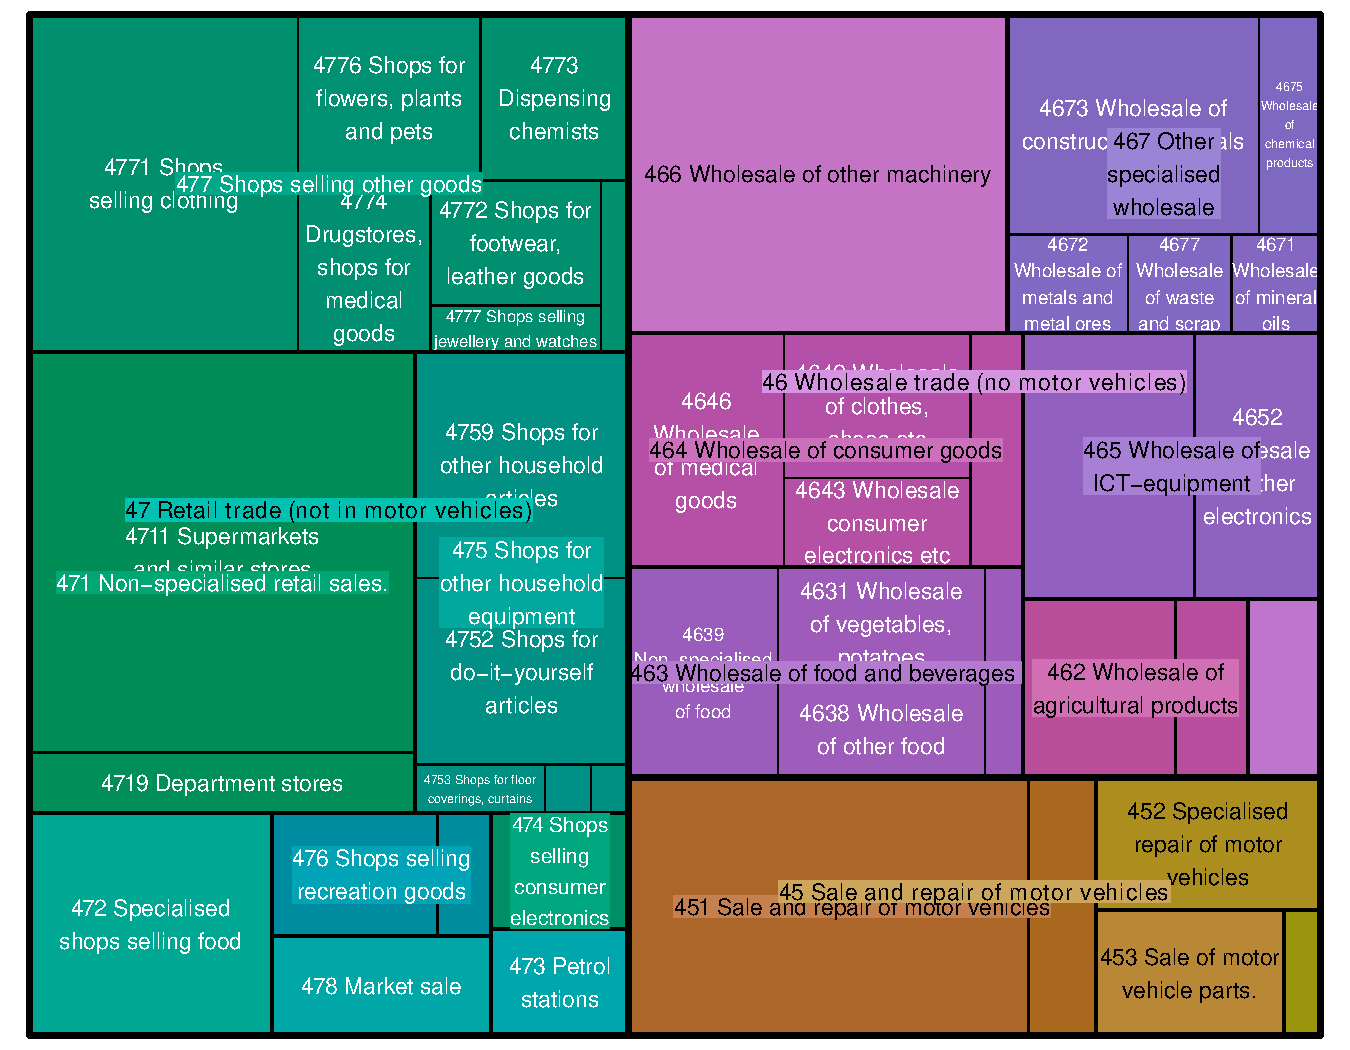
\includegraphics[width=3.5in]{TMbusiness.pdf}

  \caption{Turnover among Dutch manufacturing enterprises in 2011}\label{fig:treemapApp}

\end{figure}



\begin{figure}[htb]
  \centering
  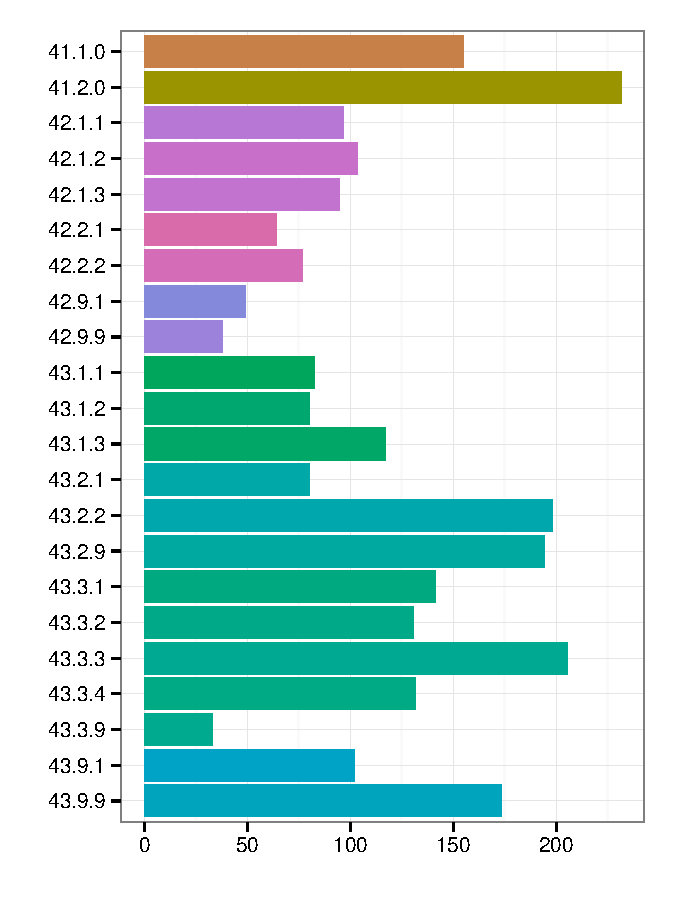
\includegraphics[width=1.235in]{bar_chart.pdf}
  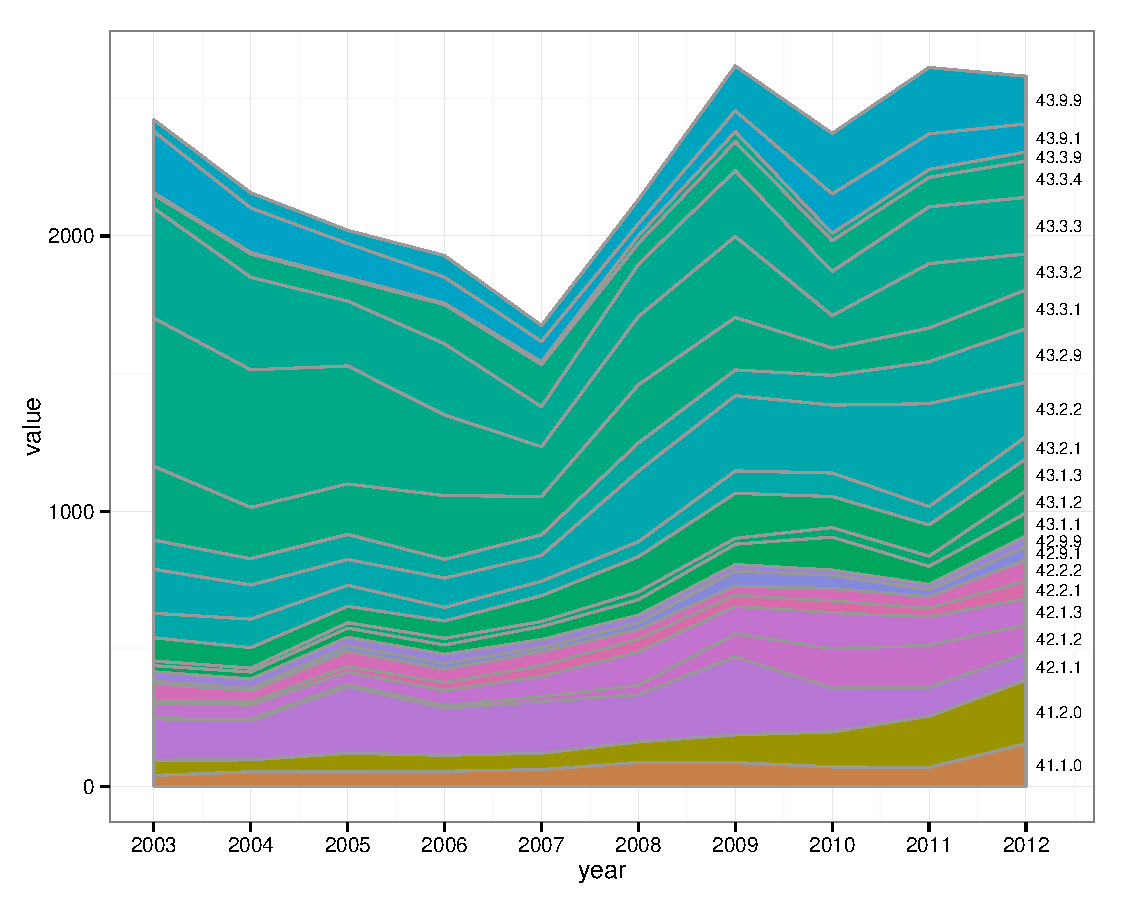
\includegraphics[width=2.065in]{stackedarea_chart.pdf}
  \caption{Bar chart and stacked area chart with hierarchical colors}\label{fig:charts}
\end{figure}

%\begin{figure}[htb]
%  \centering
%  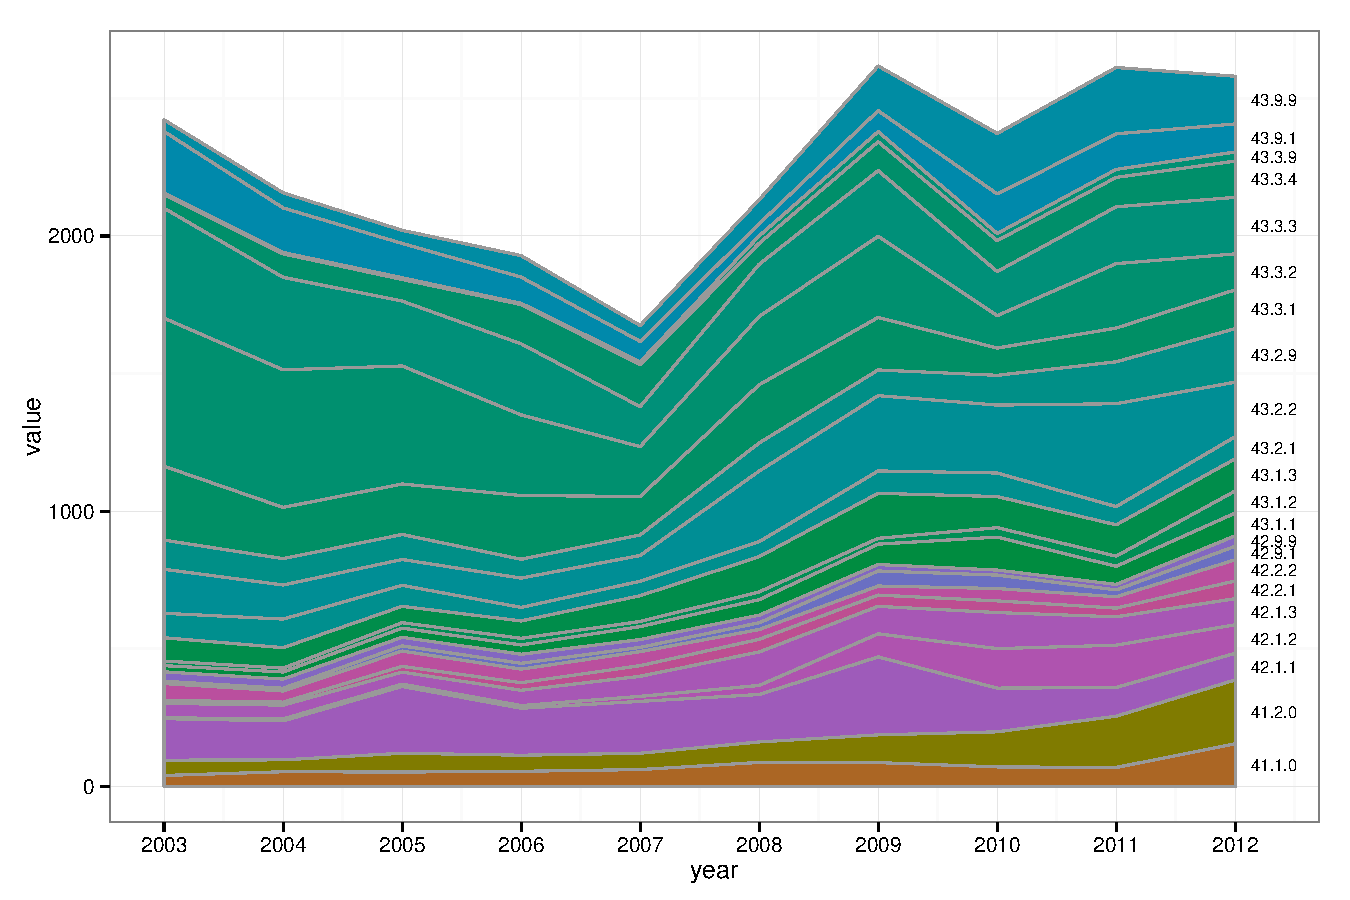
\includegraphics[width=0.25in]{stackedline_chart.pdf}
%  \caption{Stacked line chart with hierarchical colors}\label{fig:linechart}
%\end{figure}
%\begin{figure}[htb]
%  \centering
%  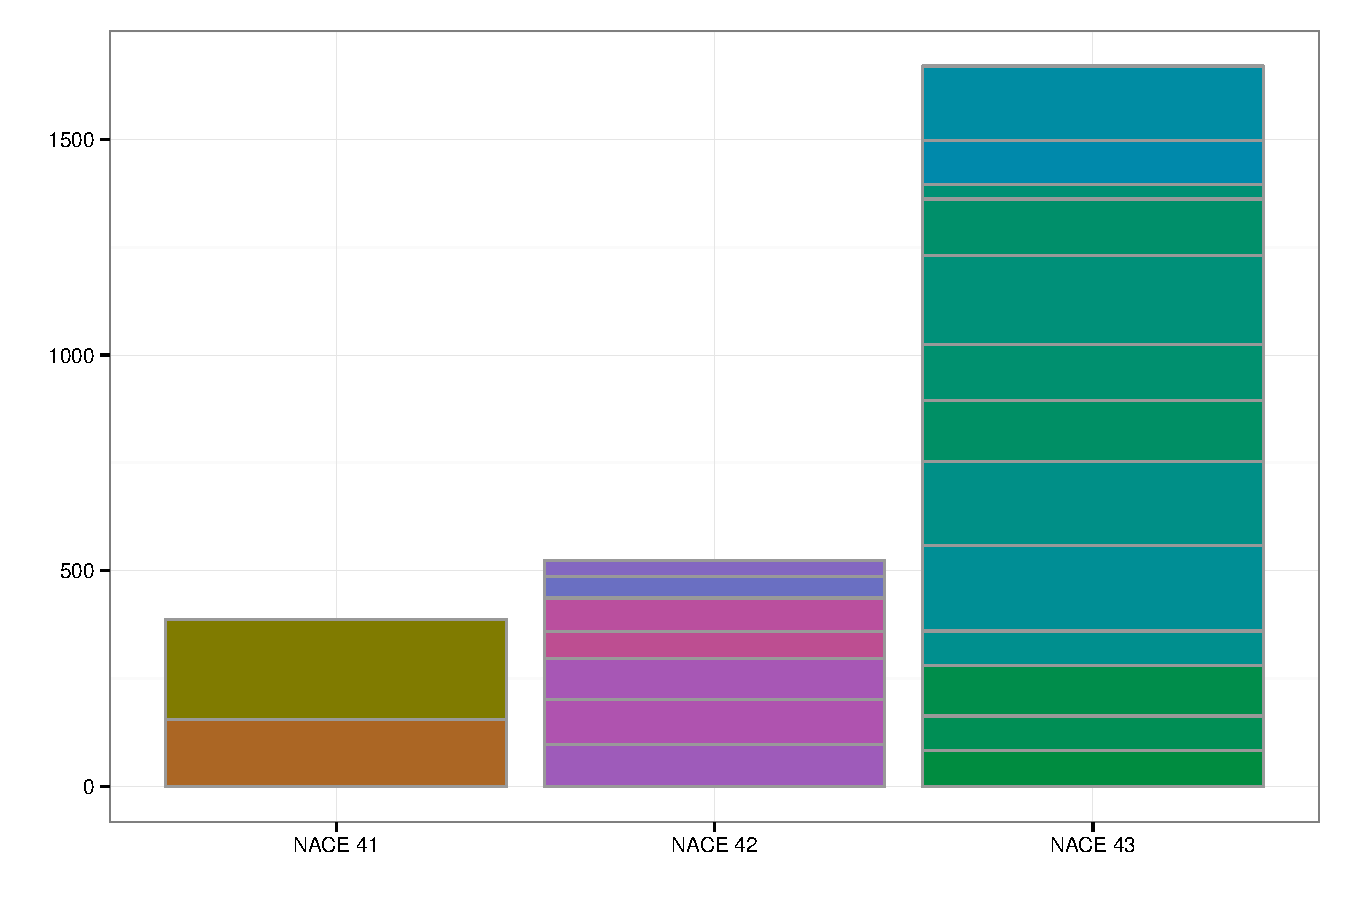
\includegraphics[width=1.75in]{stackedbar_chart.pdf}
%  \caption{Stacked bar chart with hierarchical colors}\label{fig:barchart}
%\end{figure}




\section{User study}~\label{secuser}


\section{Discussion}~\label{secdisc}
In our opinion, the proposed method to create hierarchical color palettes improves statistical visualizations, both hierarchically and non-hierarchically structured. The pre-condition that colors in the same hierarchical layer should be similar in terms of colorfulness and brightness it satisfied. This property is especially important in statistical visualizations, since they aim to visualize data as objectively as possible. The downside of the proposed method is that some leaf node colors will still be hard to distinguish.

We recommend a user study to evaluate the obtained hierarchical color palettes when applied in various statistical visualizations. The main aim of this user study would be to find out whether hierarchical palettes are useful in statistical analysis.


%% if specified like this the section will be committed in review mode
\acknowledgments{
The authors wish to thank their collegues at Statistics Netherlands who participated in the user survey.}

\bibliographystyle{abbrv}
%%use following if all content of bibtex file should be shown
%\nocite{*}
\bibliography{hcp}
\end{document}
